% !TeX spellcheck = en_US
% !TeX program = lualatex


% Do not surround the equal signs with spaces, it causes errors!
\documentclass[
	aspectratio=43,
	color={accentcolor=1c},
	logo=false,
	colorframetitle=true
]{tudabeamer}

% Include preamble to not clutter this file.
% Core packages.
% Primary: English, Secondary: German.
\usepackage[main = english, ngerman]{babel}
% Other packages.
%\usepackage{graphicx}
\usepackage{tikz}
\usepackage{mathtools}
\usepackage{amssymb}
\usepackage{siunitx}
\usepackage{amsthm}
% Remove dot at the end: nopostdot; Don't skip any groups: nogroupskip
\usepackage[xindy, section = section, nonumberlist, sanitize={symbol=false}, shortcuts, acronym, nomain, nowarn]{glossaries}
\usepackage{tabularx}
\usepackage{booktabs}
\usepackage{longtable}
\usepackage{enumitem}
%\usepackage{listings}
\usepackage{xcolor}
\usepackage{caption}
\usepackage{subcaption}
\usepackage{epstopdf}
\usepackage{wrapfig}
\usepackage[ruled, vlined, linesnumbered, resetcount, algochapter]{algorithm2e}
\usepackage[autostyle]{csquotes}
\usepackage{microtype}
\usepackage{physics}
\usepackage{cancel}
\usepackage{hyperref}
\usepackage{tabto}
\usepackage{eqparbox}
\usepackage{pgfplots}
\usepackage{multicol}
\usepackage{listings}
\usepackage{xspace}
\usepackage[bottom]{footmisc}

\usetikzlibrary{arrows.meta, shapes, backgrounds, angles, calc, chains, scopes, decorations.pathmorphing, patterns, positioning, quotes}

% Debug packages.
\usepackage{comment}
\usepackage{todonotes}

\makeatletter

% Make LOF a section.
\renewcommand\listoffigures{
	\section*{\listfigurename}
	\@mkboth{\MakeUppercase\listfigurename}{\MakeUppercase\listfigurename}
	\@starttoc{lof}
}
% Make LOT a section.
\renewcommand\listoftables{
	\section*{\listtablename}
	\@mkboth{\MakeUppercase\listtablename}{\MakeUppercase\listtablename}
	\@starttoc{lot}
}

\makeatother



% Style definitions.

% Description-list styling.
\SetLabelAlign{parright}{\parbox[t]{\labelwidth}{\raggedleft#1}}
\setlist[description]{style = multiline, leftmargin = 4cm, align = parright}

\MakeOuterQuote{"}

% Captions should be centered.
\captionsetup{justification=centering}

% Matrix/Vector notation.
\renewcommand{\vec}[1]{\boldsymbol{\mathrm{#1}}}
\newcommand{\mat}[1]{\boldsymbol{\mathrm{#1}}}
% Shorthands.
\renewcommand{\C}{\mathbb{C}}
\newcommand{\R}{\mathbb{R}}
\newcommand{\E}{\mathbb{E}}
\newcommand{\normal}{\mathcal{N}}
\newcommand{\gaussianMulti}[4]{\frac{1}{\left(2\pi\right)^{#4/2} \cdot \lvert #3 \rvert^{1/2}} \exp \bigg\{\! -\frac{1}{2} \left(#1 - #2\right)^T #3^{-1} \left(#1 - #2\right) \bigg\}}
\newcommand{\logGaussianMulti}[4]{-\frac{1}{2} \ln \lvert #3 \rvert - \frac{#4}{2} \ln\left(2\pi\right) - \frac{1}{2} \left(#1 - #2\right)^T #3^{-1} \left(#1 - #2\right)}
\newcommand{\subgiven}{\vert}
\newcommand{\given}{\,\vert\,}
\newcommand{\biggiven}{\,\big\vert\,}
\newcommand{\Biggiven}{\,\Big\vert\,}
\newcommand{\bigggiven}{\,\bigg\vert\,}
\newcommand{\Bigggiven}{\,\Bigg\vert\,}
\newcommand{\new}{\mathrm{new}}
\newcommand{\KL}[2]{D_\mathrm{KL}\big( #1 \,\Vert\, #2 \big)}
\newcommand{\SRC}{\mathit{SRC}}
% Math operators.
\DeclareMathOperator{\const}{const}
\DeclareMathOperator{\Cov}{Cov}
\DeclareMathOperator{\diag}{diag}

\newcommand{\oversetfootnotemark}[1]{\stepcounter{footnote} \overset{\mathclap{(\thefootnote)}}{#1}}
\let\realfootnote\footnote
\let\realfootnotetext\footnotetext
\renewcommand{\footnote}[1]{\realfootnote{\, #1}}
\renewcommand{\footnotetext}[1]{\realfootnotetext{\, #1}}
\newcommand{\doublefootnotetext}[2]{\addtocounter{footnote}{-1} \footnotetext{#1} \stepcounter{footnote} \footnotetext{#2}}
\newcommand{\triplefootnotetext}[3]{\addtocounter{footnote}{-2} \footnotetext{#1} \stepcounter{footnote} \footnotetext{#2} \stepcounter{footnote} \footnotetext{#3}}

\renewcommand{\arraystretch}{1.5}
\parindent0pt

% Definitions, Theorems and Lemmata.
\newtheorem{theorem}{Theorem}[chapter]
\newtheorem{definition}[theorem]{Definition}
\newtheorem{lemma}[theorem]{Lemma}

% Do not include subsections and lower in TOC.
\setcounter{tocdepth}{1}

% BibTeX.
\renewcommand{\bibname}{References}
%\bibliographystyle{ieeetr}
\bibliographystyle{alpha}

% Penalties.

% TikZ-related stuff.
\tikzset{> = { Latex[length = 2mm] }}



% Glossary styles.
\newcolumntype{L}[1]{>{\raggedright\let\newline\\\arraybackslash\hspace{0pt}}m{#1}}
\newcolumntype{C}[1]{>{\centering\let\newline\\\arraybackslash\hspace{0pt}}m{#1}}
\newcolumntype{R}[1]{>{\raggedleft\let\newline\\\arraybackslash\hspace{0pt}}m{#1}}
\newglossarystyle{iasThesisGeneral}{
	\glossarystyle{super3colheader}%
	\renewenvironment{theglossary}%
		{\begin{longtable}{L{0.15\textwidth}L{0.8\textwidth}R{0\textwidth}}}%
		{\end{longtable}}%
	\renewcommand*{\glossaryheader}{\textbf{\entryname} & \textbf{\descriptionname} & \\}
	\renewcommand*{\glossaryentryfield}[5]{\glsentryitem{##1}\glstarget{##1}{##2} & ##3 \\}
}
\newglossarystyle{iasThesisOperators}{
	\glossarystyle{super3colheader}
	\renewenvironment{theglossary}
		{\begin{longtable}{L{0.15\textwidth}L{0.55\textwidth}L{0.25\textwidth}}}%
		{\end{longtable}}%
	\renewcommand*{\glossaryheader}{\textbf{\entryname} & \textbf{\descriptionname} & \textbf{Operator} \\}
	\renewcommand*{\glossaryentryfield}[5]{\glsentryitem{##1}\glstarget{##1}{##2} & ##3 & ##4 \\}
}



\title{Variational Autoenconders for Koopman Dynamical Systems}
\subtitle{B.Sc. Intermediate Presentation}
\author{Fabian Damken}
\department{Department of Computer Science}
\institute{Intelligent Autonomous Systems}
\date{\today}

\logo*{
\includegraphics{./img/iasLogo}}

\titlegraphic*{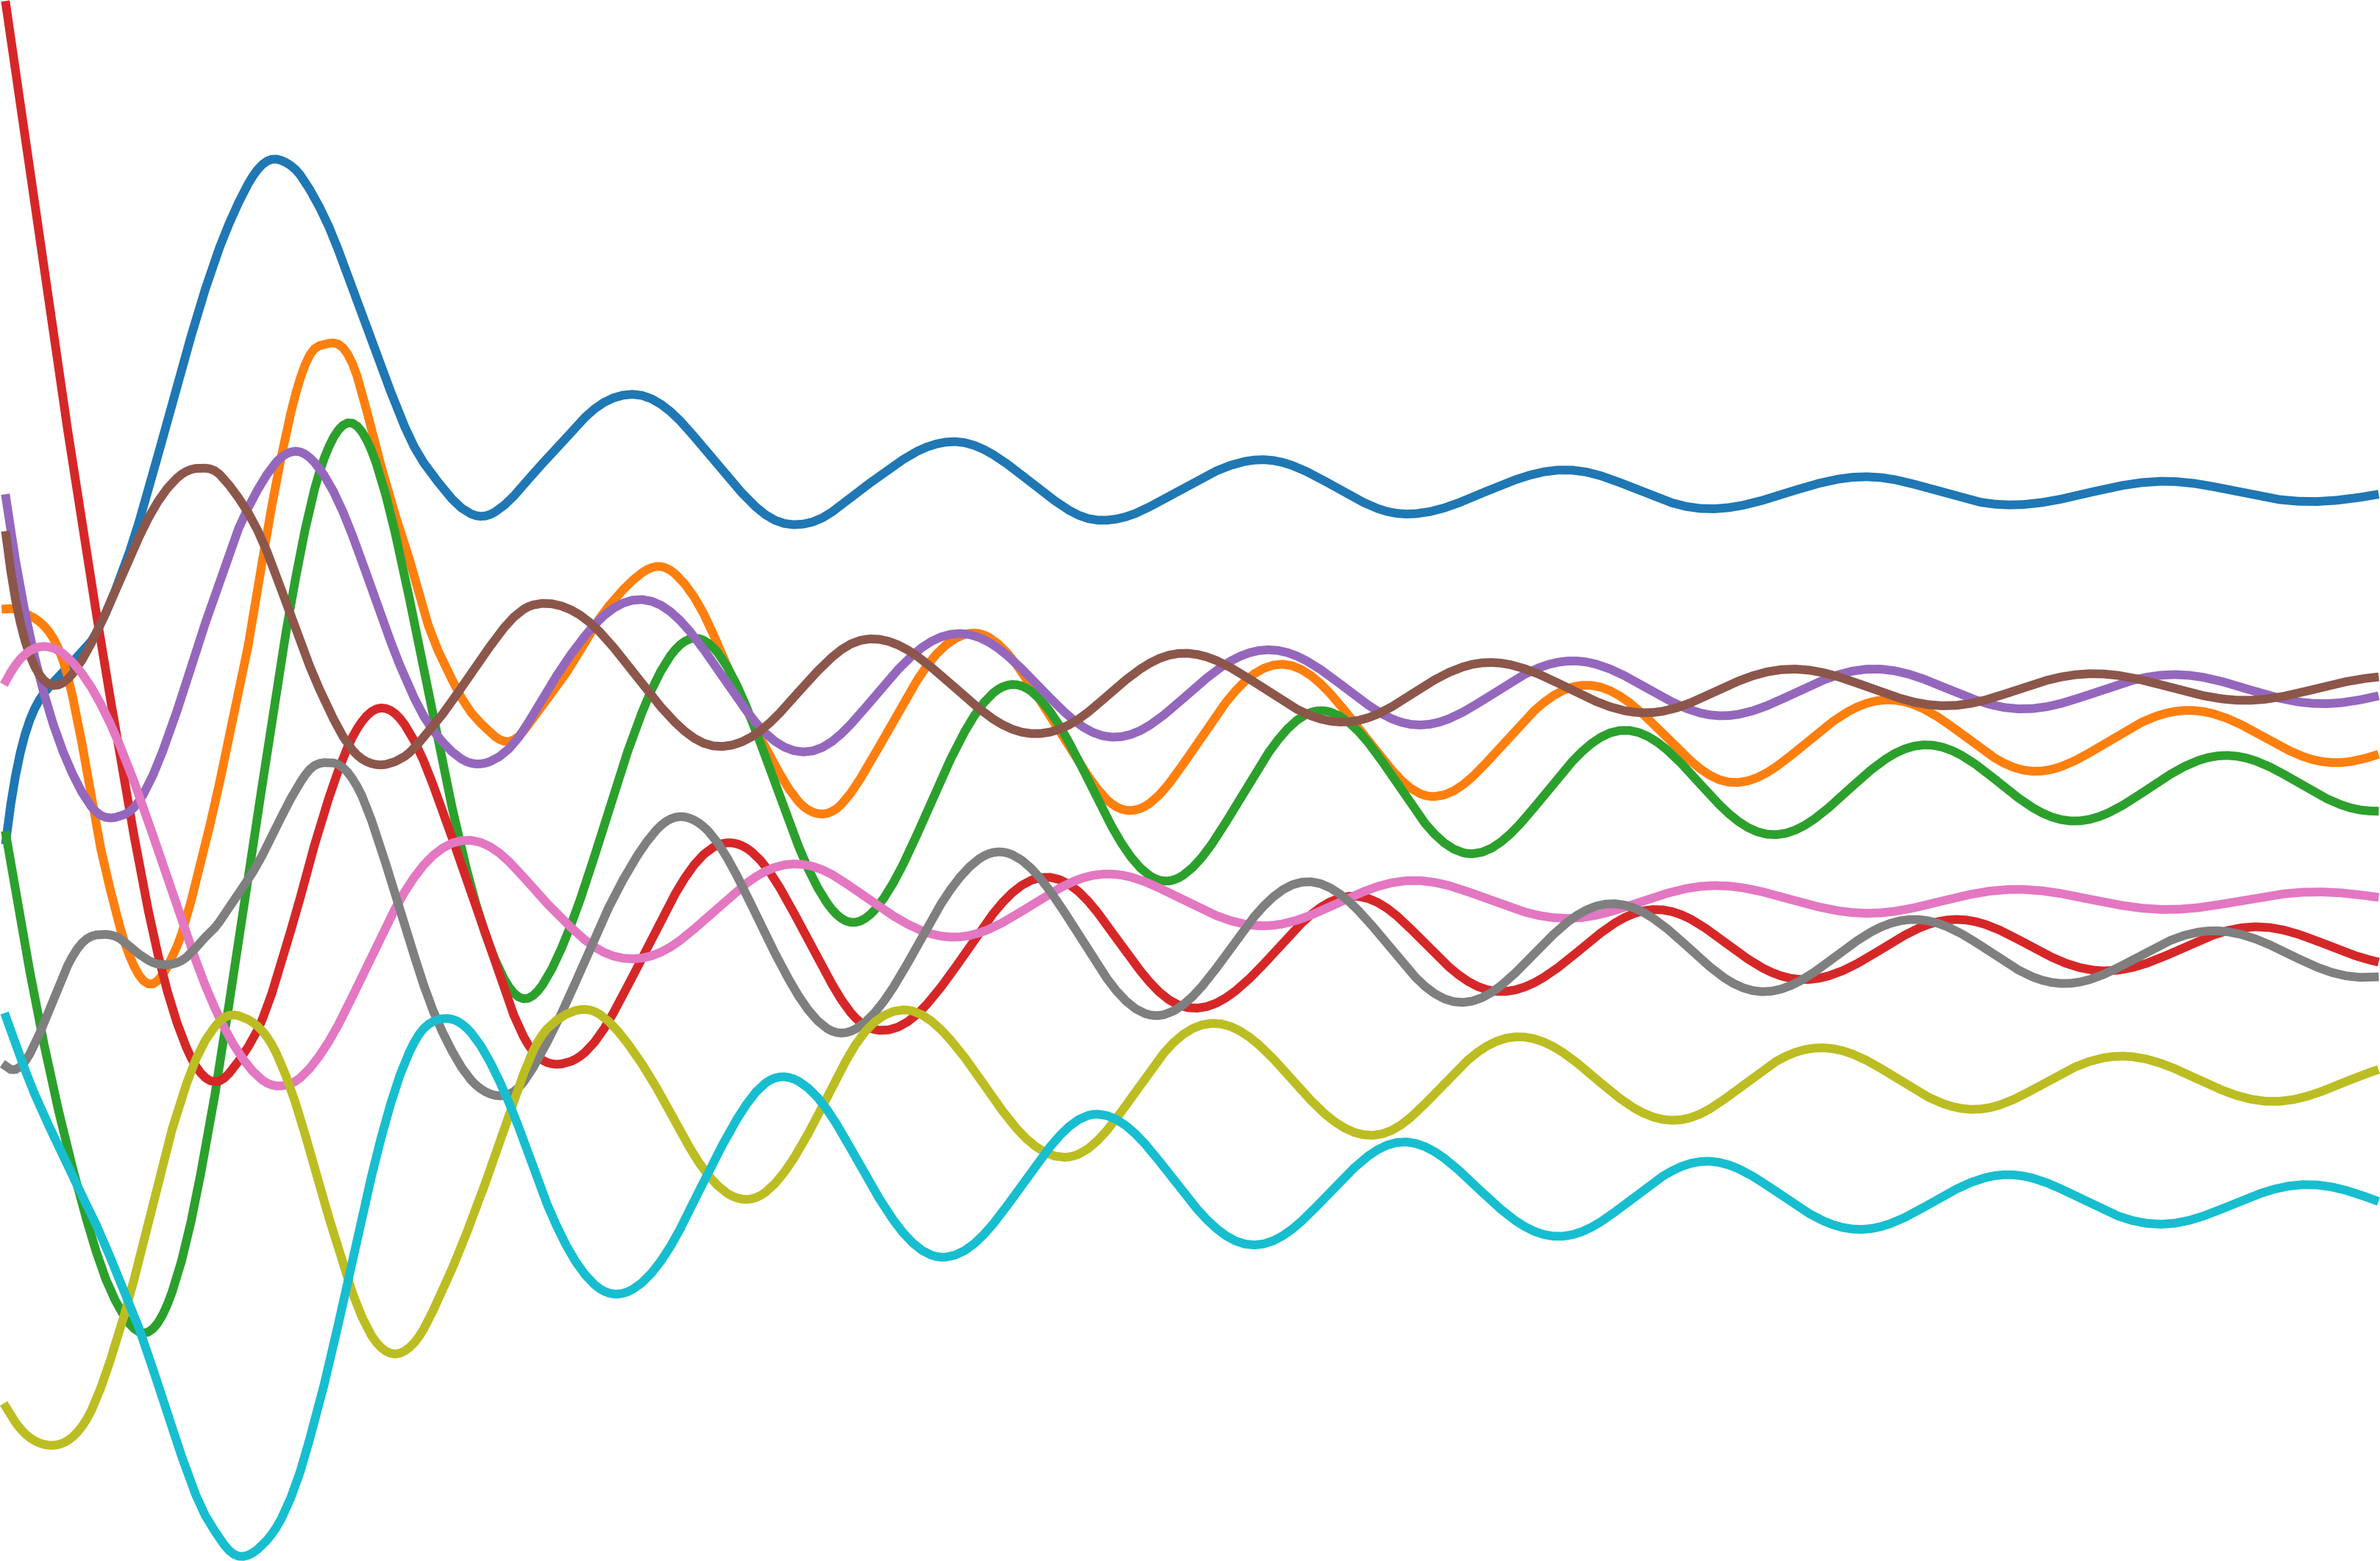
\includegraphics{figures/title}}

\begin{document}
	\maketitle

	\begin{frame}{Motivation}
		\begin{itemize}
			\item Control theory for linear systems is highly evolved.
			\item But nonlinear systems are hard\dots
			\item We need ways to linearize a nonlinear system!
			\item<2-> "Classical" Linearization:
				\begin{itemize}
					\item Use small angle approximation (e.g. for pendulum)?
					\item Diverge fast with higher displacements\dots
					\item Only linearize locally, not globally.
				\end{itemize}
			\item<3-> Koopman theory offers a way to do that!
		\end{itemize}
	\end{frame}

	\begin{frame}{The Koopman Operator}
		For a \emph{nonlinear} dynamical system
		\begin{align*}
			\vec{s}_{t + 1} = \vec{F}(\vec{s}_{t})
		\end{align*}
		with \emph{nonlinear} measurements (and \emph{embedding})
		\begin{align*}
			\vec{y}_t = \vec{g}(\vec{s}_t)
		\end{align*}
		the Koopman operator advances these measurements forward in time \emph{linearly}:
		\begin{align*}
			\vec{g}(\vec{s}_{t + 1}) = \mathcal{K} \vec{g}(\vec{s}_t)
			\quad\iff\quad
			\vec{y}_{t + 1} = \mathcal{K} \vec{y}_t
		\end{align*}

		This is possible for every nonlinear dynamical system. And globalizes linearly! But the embedding \(\vec{g}\) is typically infinite-dimensional\dots
	\end{frame}

	\begin{frame}{Koopman Dynamical System ("Deterministic")}
		\begin{figure}
			\begin{tikzpicture}[->, state/.style = { draw, circle, minimum height = 1cm, minimum width = 1cm }, observation/.style = { draw, circle, minimum height = 1cm, minimum width = 1cm }]
				\node [state] (s1) {\(\vec{s}_{\,\mathclap{\,1}}\)};
				\node [state, right = 1 of s1] (s2) {\(\vec{s}_{\,\mathclap{\,2}}\)};
				\node [state, right = 1 of s2] (s3) {\(\vec{s}_{\,\mathclap{\,3}}\)};
				\node [minimum height = 1cm, right = 1 of s3] (sD) {\(\cdots\)};
				\node [state, right = 1 of sD] (sT) {\(\vec{s}_{\,\mathclap{\,T}}\)};

				\node [observation, below = 1 of s1] (y1) {\raisebox{-5pt}{\(\vec{y}_{\,\mathclap{\,1}}\)}};
				\node [observation, below = 1 of s2] (y2) {\(\vec{y}_{\,\mathclap{\,2}}\)};
				\node [observation, below = 1 of s3] (y3) {\(\vec{y}_{\,\mathclap{\,3}}\)};
				\node [minimum height = 1cm, below = 1 of sD] (yD) {\(\cdots\)};
				\node [observation, below = 1 of sT] (yT) {\(\vec{y}_{\,\mathclap{\,T}}\)};

				\draw (s1) -- node[above]{\(\vec{F}\)} (s2);
				\draw (s2) -- node[above]{\(\vec{F}\)} (s3);
				\draw (s3) -- node[above]{\(\vec{F}\)} (sD);
				\draw (sD) -- node[above]{\(\vec{F}\)} (sT);

				\draw (y1) -- node[below]{\(\mathcal{K}\)} (y2);
				\draw (y2) -- node[below]{\(\mathcal{K}\)} (y3);
				\draw (y3) -- node[below]{\(\mathcal{K}\)} (yD);
				\draw (yD) -- node[below]{\(\mathcal{K}\)} (yT);

				\draw (s1) to[bend right = 15] node[left]{\(\vec{g}\)} (y1);
				\draw (s2) to[bend right = 15] node[left]{\(\vec{g}\)} (y2);
				\draw (s3) to[bend right = 15] node[left]{\(\vec{g}\)} (y3);
				\draw (sT) to[bend right = 15] node[left]{\(\vec{g}\)} (yT);

				\draw [dashed] (y1) to[bend right = 15] node[right]{\(\vec{g}^{-1}\)} (s1);
				\draw [dashed] (y2) to[bend right = 15] node[right]{\(\vec{g}^{-1}\)} (s2);
				\draw [dashed] (y3) to[bend right = 15] node[right]{\(\vec{g}^{-1}\)} (s3);
				\draw [dashed] (yT) to[bend right = 15] node[right]{\(\vec{g}^{-1}\)} (sT);
			\end{tikzpicture}
			\caption{Adopted from Brunton et al. "Koopman Invariant Subspaces and Finite Linear Representations of Nonlinear Dynamical Systems for Control".}
		\end{figure}
	\end{frame}

	\begin{frame}{Linear Gaussian Dynamical System}
		\begin{figure}
			\begin{tikzpicture}[->, state/.style = { draw, circle, minimum height = 1cm, minimum width = 1cm }, observation/.style = { draw, circle, minimum height = 1cm, minimum width = 1cm }]
				\node [state] (s1) {\(\vec{s}_{\,\mathclap{\,1}}\)};
				\node [state, right = 1 of s1] (s2) {\(\vec{s}_{\,\mathclap{\,2}}\)};
				\node [state, right = 1 of s2] (s3) {\(\vec{s}_{\,\mathclap{\,3}}\)};
				\node [minimum height = 1cm, right = 1 of s3] (sD) {\(\cdots\)};
				\node [state, right = 1 of sD] (sT) {\(\vec{s}_{\,\mathclap{\,T}}\)};

				\node [observation, below = 1 of s1] (y1) {\raisebox{-5pt}{\(\vec{y}_{\,\mathclap{\,1}}\)}};
				\node [observation, below = 1 of s2] (y2) {\(\vec{y}_{\,\mathclap{\,2}}\)};
				\node [observation, below = 1 of s3] (y3) {\(\vec{y}_{\,\mathclap{\,3}}\)};
				\node [observation, below = 1 of sT] (yT) {\(\vec{y}_{\,\mathclap{\,T}}\)};

				\draw (s1) -- (s2);
				\draw (s2) -- (s3);
				\draw (s3) -- (sD);
				\draw (sD) -- (sT);

				\draw (s1) to[bend right = 15] (y1);
				\draw (s2) to[bend right = 15] (y2);
				\draw (s3) to[bend right = 15] (y3);
				\draw (sT) to[bend right = 15] (yT);

				\draw [dashed] (y1) to[bend right = 15] (s1);
				\draw [dashed] (y2) to[bend right = 15] (s2);
				\draw [dashed] (y3) to[bend right = 15] (s3);
				\draw [dashed] (yT) to[bend right = 15] (sT);
			\end{tikzpicture}
		\end{figure}

		\begin{equation*}
			\begin{aligned}
				\vec{s}_{t + 1} &= \eqmakebox[a][l]{\( \mat{A} \vec{s}_t + \vec{v}, \)}\quad \eqmakebox[b][r]{\( \vec{v} \)} \sim \normal(\vec{0}, \mat{Q}) \\
				\vec{y}_t &= \eqmakebox[a][l]{\( \vec{g}_{\vec{\theta}}(\vec{s}_t) + \vec{w}, \)}\quad \eqmakebox[b][r]{\( \vec{w} \)} \sim \normal(\vec{0}, \mat{R})
			\end{aligned}
			\qquad\iff\qquad
			\begin{aligned}
				\vec{s}_{t + 1} &\sim \normal(\mat{A} \vec{s}_t, \mat{Q}) \\
				\vec{y}_t &\sim \normal(\vec{g}_{\vec{\theta}}(\vec{s}_t), \mat{R})
			\end{aligned}
		\end{equation*}
	\end{frame}

	\begin{frame}{How to learn?}
		Goal: Estimate all of the following:
		\begin{itemize}
			\item Latent dynamics matrix \( \mat{A} \).
			\item Measurement function \( \vec{g}_{\vec{\theta}}(\cdot) \) (i.e. the parameters \( \vec{\theta} \)). \\ Variational auto-encoder without an amortization network.
			\item Noise covariances \(\mat{Q}\), \(\mat{R}\).
		\end{itemize}
		We employ an EM-algorithm to do that.

		\onslide<2->{
			\begin{alertblock}{Core Problem}
				Some expectations cannot be evaluated in closed form for a nonlinear \( \vec{g}_{\vec{\theta}}(\cdot) \).
			\end{alertblock}
		}

		\onslide<3->{
			\begin{itemize}
				\item Use cubature rules for evaluating the intractable expectations.
				\item No closed form solution for maximizing w.r.t. function parameters \( \vec{\theta} \).
				\item<4->[] \(\qquad\longrightarrow\quad\) Use backpropagation and gradient descent!
			\end{itemize}
		}
	\end{frame}

%	\begin{frame}{Relation to the Evidence Lower Bound (ELBO)}
%		\begin{align*}
%			\mathcal{L}_{\text{ELBO}}(\vec{\theta}, \vec{\phi}; \vec{x}) = \E_{q_{\vec{\phi}}(\vec{z} \subgiven \vec{x})} \big[\! \ln p_{\vec{\theta}}(\vec{x} \given \vec{z}) \big] - D_\mathrm{KL}\big( q_{\vec{\phi}}(\vec{z} \given \vec{x}) \,\Vert\, p_{\vec{\theta}}(\vec{z}) \big)
%		\end{align*}
%	\end{frame}

	\section{Results}
		\subsection{The Pendulum}
			\begin{frame}{Results: Damped Inverted Pendulum \\ Dynamical System}
				\vspace{-0.7cm}
				\begin{align*}
					\ddot{\varphi} = \frac{g}{L} \sin(\varphi) - d \dot{\varphi}
					\quad\longrightarrow\quad
					\ddot{\varphi} = \sin(\varphi) - 0.1 \dot{\varphi}
				\end{align*}

				\begin{minipage}{0.34\textwidth}
					Observations:
					\begin{itemize}
						\item Displacement \tabto{2.5cm} \(\varphi\)
						\item Velocity     \tabto{2.5cm} \(\dot{\varphi}\)
					\end{itemize}
					\begin{figure}
						\centering
						\begin{tikzpicture}
							\node [draw, circle, fill, minimum width = 0.5cm] (C) at (0, 0) {};
							\node [draw, circle] (mass) at (120:3cm) {\(m\)};
							\coordinate (A) at (90:3cm);
							\draw (C) -- node[left]{\(L\)} (mass);
							\draw [dashed] (C) -- (A);
							\draw pic [draw, angle radius = 1.5cm] {angle=A--C--mass};
							\node at (-0.27, 1.0) {\(\varphi\)};

							\draw [<-] (0.5, 1) -- node[right]{\(g\)} (0.5, 2);
						\end{tikzpicture}
					\end{figure}
				\end{minipage}
				\begin{minipage}{0.65\textwidth}
					\begin{figure}
						\centering
						\onslide<2->{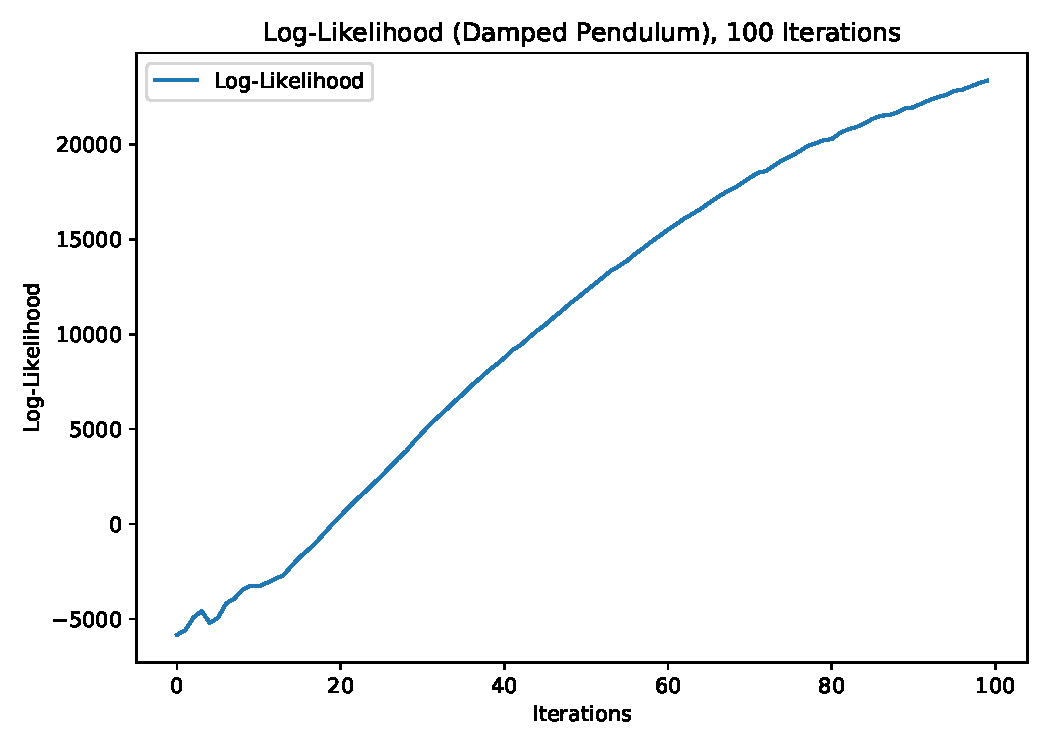
\includegraphics[width=\textwidth]{figures/results/log-likelihood}}
					\end{figure}
				\end{minipage}
			\end{frame}

			\begin{frame}{Results: Damped Inverted Pendulum \\ Rollout/Prediction in Observation Space, 10 Latents}
				\vspace{-0.4cm}
				\begin{figure}
					\centering
					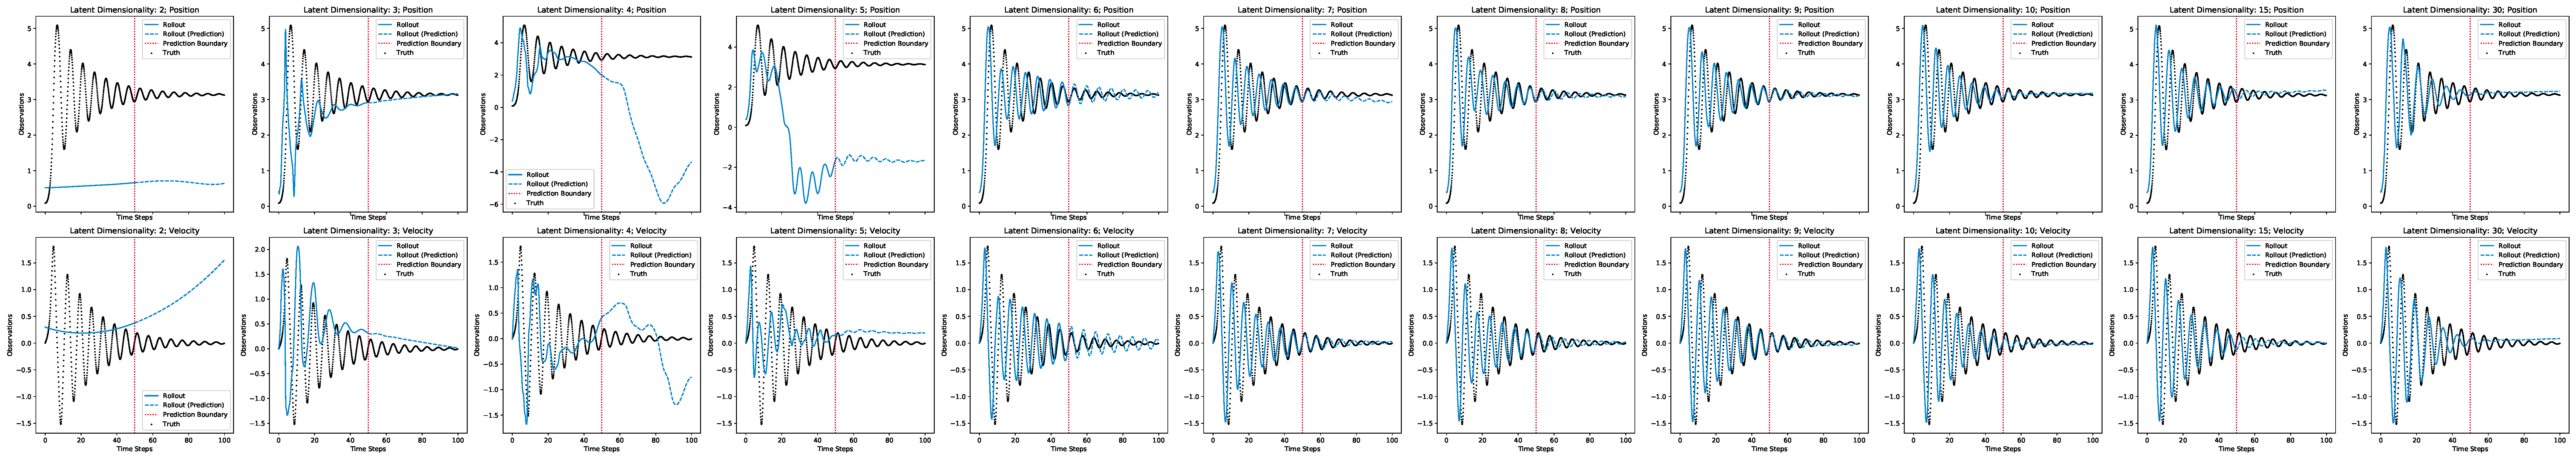
\includegraphics[height = 0.8\textheight]{figures/results/latent-dimensions-experiment_rollout}
				\end{figure}
			\end{frame}

			\begin{frame}{Results: Damped Inverted Pendulum \\ Different Sizes of Latent Dimension}
				\vspace{-0.4cm}
				\begin{figure}
					\centering
					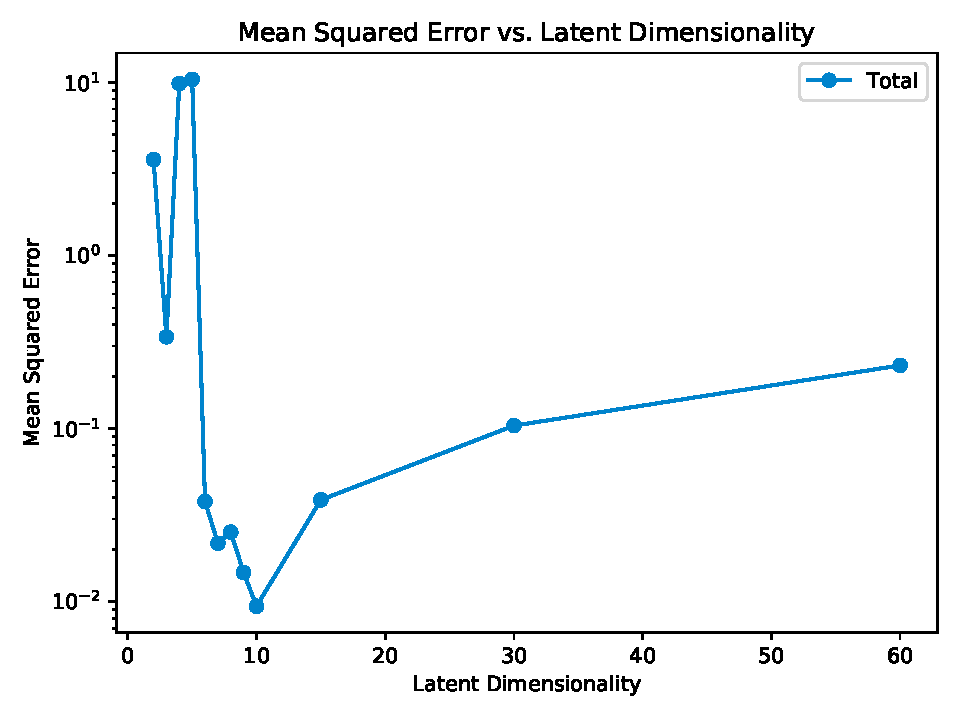
\includegraphics[height = 0.8\textheight]{figures/results/latent-dimensions-experiment_mse}
				\end{figure}
			\end{frame}
		% end
	% end

	\section{Related Work and Outlook}
		\begin{frame}{Related Work}
			\begin{itemize}
				\item<+-> Lusch et al. "Deep Learning for Universal Linear Embeddings of Nonlinear Dynamics":
					\begin{itemize}
						\item Use an autoencoder approach with an encoder network.
						\item No probabilistic interpretation.
					\end{itemize}
				\item<+-> Morton et al. "Deep Variational Koopman Models: Inferring Koopman Observations for Uncertainty-Aware Dynamics Modeling and Control":
					\begin{itemize}
						\item Utilize six different neural networks to perform variational inference.
						\item We use only one!
						\item And we expect to do at least as good.
					\end{itemize}
				\item<+-> Becker et al. "Recurrent Kalman Networks: Factorized Inference in High-Dimensional Deep Feature Spaces"
				\item<+-> Zhang, Vikram et al. "SOLAR: Deep Structured Representations for Model-Based Reinforcement Learning"
			\end{itemize}
		\end{frame}

		\begin{frame}{Hypothesis and Outlook}
			\begin{itemize}
				\item Tackle the ELBO using approximate EM rather than stochastic variational inference.
				\item Assume we can do at least as good as Morton et al. with simpler network architectures.
				\item Perform control tasks on pendulum, cartpole, acrobot.
			\end{itemize}
		\end{frame}
	% end





	\appendix

	\section{Backup Slides} \sectionslide
		\subsection{Expectation Maximization}
			\begin{frame}{Expectation Maximization}
				\begin{itemize}
					\item E-Step: Calculate the expected latents and correlations using filtering/smoothing.
					\item M-Step: Maximize the expected log-likelihood \( \E\big[\! \ln p(\vec{s}_{1:T}, \vec{y}_{1:T}) \given \vec{y}_{1:T} \big] \).
				\end{itemize}
			\end{frame}
		% end

		\subsection{The Expected Log-Likelihood}
			\begin{frame}{The Expected Log-Likelihood}
				Markov property yields complete log-likelihood:
				\begin{align*}
					\ln p(\vec{s}_{1:T}, \vec{y}_{1:T}) = \ln p(\vec{s}_1) + \sum_{t = 2}^{T} \ln p(\vec{s}_{t + 1} \given \vec{s}_t) + \sum_{t = 1}^{T} \ln p(\vec{y}_t \given \vec{s}_t)
				\end{align*}
				Expectation \( \E\big[\! \ln p(\vec{s}_{1:T}, \vec{y}_{1:T}) \given \vec{y}_{1:T} \big] \) is based on five other expectations:
				\begin{align*}
					\hat{\vec{s}}_t \coloneqq \E\big[ \vec{s}_t \biggiven \vec{y}_{1:T} \big]
					\qquad
					\mat{P}_t \coloneqq \E\big[ \vec{s}_t \vec{s}_t^T \biggiven \vec{y}_{1:T} \big]
					\qquad
					\mat{P}_{t, t - 1} \coloneqq \E\big[ \vec{s}_t \vec{s}_{t - 1}^T \biggiven \vec{y}_{1:T} \big]
				\end{align*}
				\begin{align*}
					\hat{\vec{g}}_t \coloneqq \E\big[ \vec{g}(\vec{s}_t) \biggiven \vec{y}_{1:T} \big]
					\qquad
					\mat{G}_t \coloneqq \E\big[ \vec{g}(\vec{s}_t) \, \vec{g}^T\!(\vec{s}_t) \biggiven \vec{y}_{1:T} \big]
				\end{align*}
			\end{frame}
		% end

		\subsection{Cubature Rules}
			\begin{frame}{Quadrature for High Dimensions: Cubature Rules \\ The Spherical-Radial Cubature Rule}
				Approximation of an arbitrary Gaussian expectation:
				\begin{align*}
					\E_{\vec{x} \,\sim\, \normal(\vec{\mu}, \mat{\Sigma})}\big[ \vec{f}(\vec{x}) \big]
						&= \int_{\R^n} \! \vec{f}(\vec{x}) \, \normal(\vec{x} \given \vec{\mu}, \mat{\Sigma}) \dd{\vec{x}} \\
						&\approx \frac{1}{2n} \sum_{i = 1}^{2n} \vec{f}\Big(\! \sqrt{\mat{\Sigma}} \vec{\xi}_i + \vec{\mu} \Big),\quad \vec{\xi}_i = \sqrt{n} [\vec{1}]_i
				\end{align*}
				This finite sum can be evaluated!
			\end{frame}
		% end
	% end


	% Classical approach.
	% Interpretation as markov process or hidden markov model.
	% Probabilistic interpretation.
	% Variational approach.
	% EM algorithm.
	% Maximization goal (log-likelihood).
	% Computation via FilterinTaken fromg/Smoothing and SGD.
\end{document}
